\chapter{Implementación}
En este capitulo se describe a detalle el proceso de implementación de los diferentes módulos que forman parte del sistema  de video-vigilancia inteligente.

\section{Módulo de Cámara}

\subsection{Fuente de fotogramas}
\subsubsection{Webcam}
\subsubsection{Raspberry-picam}
\subsection{Configuración}
\subsection{Interfaz gráfica de usuario}

Referenciando a la figura \ref{fig:camera_screen}.
\begin{figure}[H]
    \begin{center}
        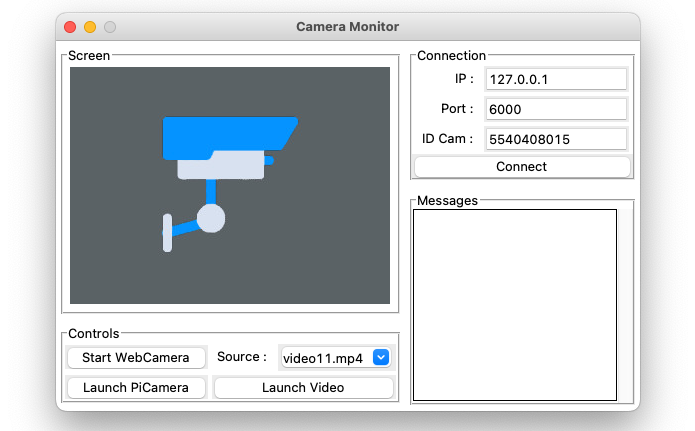
\includegraphics[width=13cm]{img/capitulo_5/camera_screen.png}
        \caption{Interfaz de la camara desarrollada.}
        Fuente : Elaboración Propia.
        \label{fig:camera_screen}
    \end{center}
\end{figure}

Referenciando a la figura \ref{fig:camera_screen}.
\begin{figure}[H]
    \begin{center}
        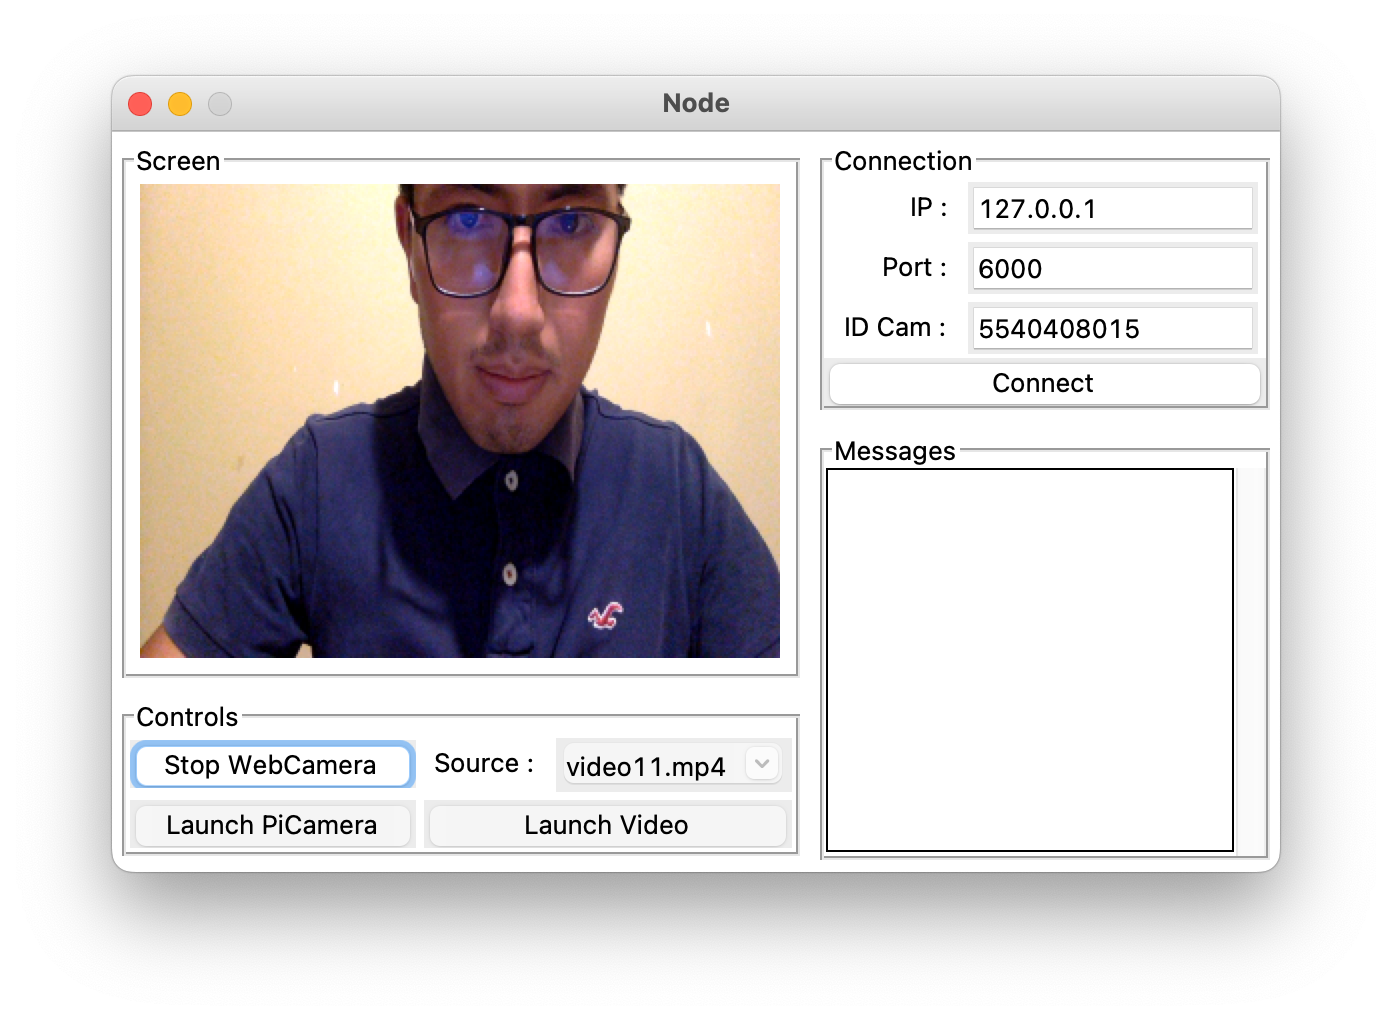
\includegraphics[width=13cm]{img/capitulo_5/webcamera.png}
        \caption{Diagrama de Gannt.}
        Fuente : Elaboración propia
        \label{fig:webcamera}
    \end{center}
\end{figure}

Referenciando a la figura \ref{fig:securityvideo}.
\begin{figure}[H]
    \begin{center}
        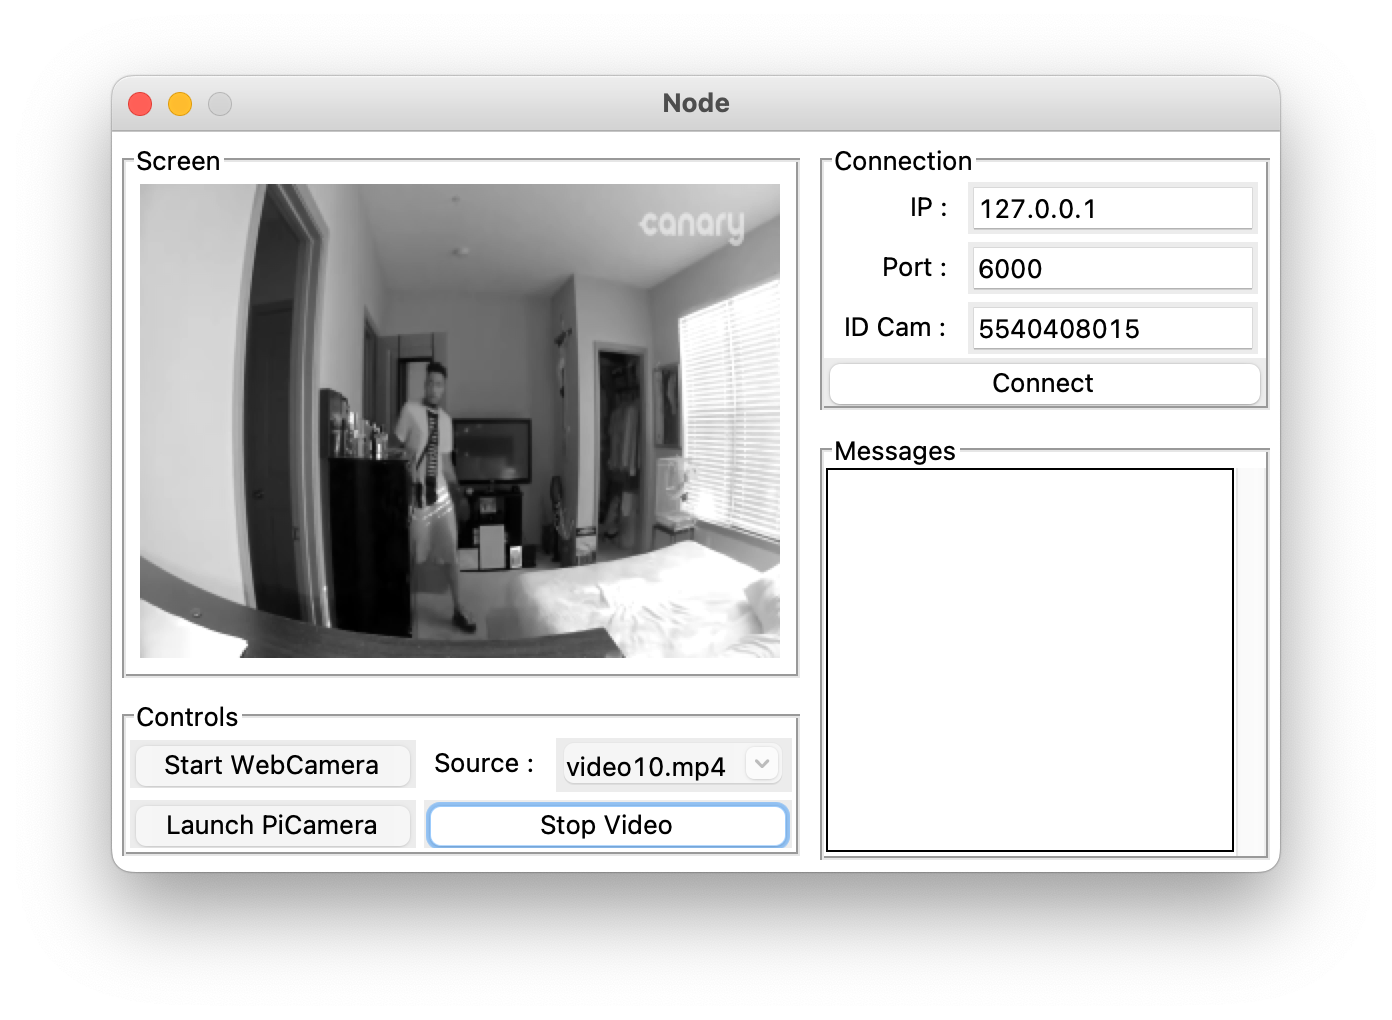
\includegraphics[width=13cm]{img/capitulo_5/security-video.png}
        \caption{Diagrama de Gannt.}
        Fuente : Elaboración propia
        \label{fig:securityvideo}
    \end{center}
\end{figure}

\subsection{Conexión al servidor}

\section{Módulo de Servidor}
\subsection{Interfaz de usuario}
Referenciando a la figura \ref{fig:servertcp_console}.
\begin{figure}[H]
    \begin{center}
        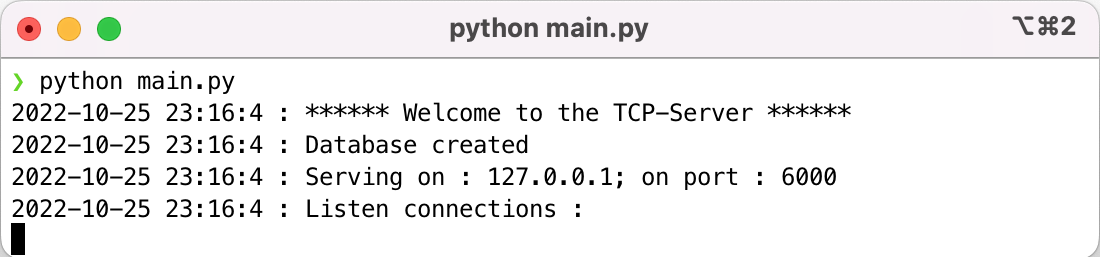
\includegraphics[width=15cm]{img/capitulo_5/tcp_server.png}
        \caption{Ejecución del servidor TCP.}
        Fuente : Elaboración propia
        \label{fig:servertcp_console}
    \end{center}
\end{figure}

\subsection{Manejador de conexiones}

\subsection{Análisis de fotogramas}
\subsubsection{Fuego y humo}
\subsubsection{Silueta humana}
\subsubsection{Movimiento}
\subsection{Streamming Http}
\section{Notificación por correo electrónico}